\section{Nuclear structure models}
\label{sec:models}
\subsection{Phenomenology of the NN interaction}
The study of low energy hadron physics, has always been a challenging task. This is due to the known fact that the strong force, which is responsible for the attraction between the nucleons in a nuclei, is not perturbative at low energies, as opposed to the atomic case for the Coulomb interaction.
It is possible nevertheless, to obtain a good description of the nuclear structure, by using empirical data obtained experimentally.
\subsubsection{Binding energies}
Let us start by the omnipresent physical quantity that is the binding energy of a nucleus. We can define it as the mass defect of the nucleus with respect to the constituents - protons and neutrons - isolated from eachother. If Z is the number of protons, N the number of neutrons, and $A=N+Z$ the nuclear mass, then the binding energy $E_B$ is given by
\begin{equation}
    \label{eq:binding_energy}
    E_B = (Zm_p + Nm_n - M)c^2
\end{equation}
where $m_p$ is the proton mass, $m_n$ the neutron mass, and $M$ the nucleus mass.
\\In figure \ref{fig:BE}, the binding energy per nucleon $E_B/A$ of nuclei as a function of $A$ is plotted. As shown in the figure, the binding energy per nucleon rapidly saturates and stalls around $7$ MeV just after $A=4$, this striking behaviour is due to nucleons interacting only with near neighbours, since the strong force is a short-range interaction, otherwise, the trend would follow a behaviour of $A(A-1)$ as in the Coulomb case.
\begin{figure}[H]
    \centering
    \includegraphics[width=0.6\textwidth]{Images/BE.png}
    \caption{Binding energy of nuclei as a function of $A$.}
    \label{fig:BE}
\end{figure}
\subsubsection{Nuclear density}
An important aspect of nuclear phenomenology which can be easily obtained through electron scattering experiments \cite{Hofstadter1956} is the nuclear density. It can be very well represented by a Fermi-like distribution, which reads
\begin{equation}
    \label{eq:phen_density}
    \rho(r)=\frac{\rho_0}{1+e^{\frac{r-R_0}{a}}},
\end{equation}
where $R_0$ is the nuclear radius, which can be parametrized as $R_0=r_0 A^{1/3}\approx 1.2A^{1/3}$, and $a$ is the diffusivity, whose value determines how sharp the density drops from its saturation value $\approx \rho_0$ to $\approx 0$. The saturation density $\rho_0$ is generally universal for all nuclei amounting to $\approx 0.16$ fm$^{-3}$.
\subsection{Nuclear models}
The description of nuclear structure has been proven to be a difficult task over the years. Due to the extremely rich phenomenology of nuclei and the challenges brought by the strong force, as we shall see, many models and further approximations to give a satisfactory description of all nuclides have been proposed.
\subsection{Liquid drop model}
One, if not the first successful model, is the liquid drop model. It is based on the assumption that the nucleus behaves as a liquid droplet, where forces among consituents tend to saturate. This hypothesis, formulated by G. Gamow culminated in the formalization of the semi-empirical mass formula (SEMF) by N. Bohr and C. F. von Weizsäcker in 1935 \cite{Weizsacker1935}, which reads
\begin{equation}
    \label{eq:semf}
    E_B=a_V A - a_S A^{2/3} - a_C \frac{Z(Z-1)}{A^{1/3}} - a_A \frac{(N-Z)^2}{A} + \delta_P
\end{equation}
where $E_B$ is the binding energy of the nucleus. Each term has a different physical and phenomenological meaning:
\begin{itemize}
    \item $a_V A$ is the volume energy of the nucleus, given by the approximately constant binding energy per nucleon, which makes the total energy roughly proportional to $A$;
    \item $a_S A^{2/3}$ is the surface energy, a correction to the volume energy due to outer nuclei -- on the surface -- interacting with fewer nucleons than those in the inner bulk;
    \item $a_C Z(Z-1)/A^{1/3}$ is the approximation to the Coulomb energy repulsion of the nucleus, assuming the protons are distributed uniformly;
    \item $a_A (N-Z)^2/A$ is the asymmetry energy, which is due to the Pauli exclusion principle, since protons and neutrons occupy their respective states, a high imbalance of one species or the other implies loosely bound nucleons, thus a higher energy contribution of those states; and
    \item $\delta_P$ refers to the pairing energy of the nucleus, whose physical significance will be later discussed in section \ref{sec:pairing_intro}.
\end{itemize}
\begin{figure}[h]
    \centering
    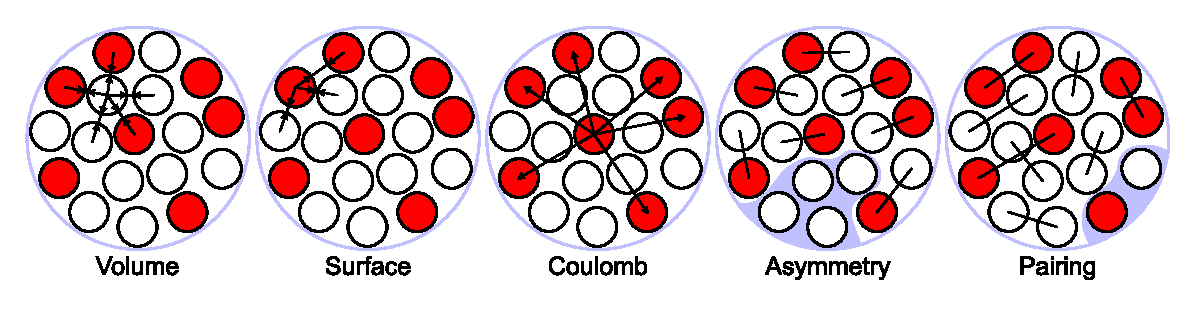
\includegraphics[width=1.0\textwidth]{Images/Liquid_drop_model.pdf}
    \caption{Visual representation of the liquid drop model from \cite{ldmimg}}
    \label{fig:liquid_drop_model}
\end{figure}
The SEMF can be fitted on current data to get a good estimate of binding energies \cite{Benzaid2020}, but it still lacks the ability of describing many aspects of nuclear structure, mainly, the nuclear shell structure, which can account for magic numbers, nuclear deformations, and so on.
\subsection{Shell structure}
The shell model, accounts for the effect of a mean field, central potential, to which nucleons are subjected. Unlike the `atomic' case, we don't have an exact source of this field, since it's generated by the nucleons themselves. Nonetheless, the formulation of a potential which reproduces experimental data has been proven to be successful.
\\The so called Woods-Saxon potential is the empirical field used in this kind of model. It can take different parametrizations depending on the data that one wants to reproduce. It reads
\begin{equation}
    \label{eq:sphWS}
    U(\bm r) = -\frac{U_0(A, N)}{1+e^\frac{r - R}{a}}
\end{equation}
where $U_0$ is the potential depth
\begin{equation}
    U_0(A, N) = U_0\bigg(1\pm \kappa \frac{2N -A }A\bigg)
\end{equation}
where the $+$ and $-$ signs refer to protons and neutrons respectively. $R$ refers to the radius of the nuclear surface, generally parametrized as 
\begin{equation}
    R=r_0 A^{1/3}
\end{equation}
and $a$ is the surface diffuseness, as in the density expression in \eqref{eq:phen_density}, which motivates the reason for such a construction in equation \eqref{eq:sphWS}, it has the shape of the nuclear density.
\paragraph{Spin-orbit coupling} 
The success of the shell model is due to the possibility of accounting for spin-orbit interactions, included through a term which reads
\begin{equation}
    U_{\text{LS}}(\bm r )=U_0^{\text{LS}}\bigg(\frac{r_0}{\hbar}\bigg)^2 \frac 1 r \dv{}{r}\bigg (\frac{1}{1+e^{\frac{r-R}{a}}}\bigg).
\end{equation}
\paragraph{Coulomb interaction}
In the spherical case, the coulomb interaction can be taken as the energy potential produced by a sphere of charge $Z$ and radius $R$, which reads
\begin{equation}
    U_{\text{C}}(r) = Ze^2
    \begin{cases}
        \frac{3-(r/R)^2}{2R} & r \le R \\
        \frac 1 r & r > R
    \end{cases}
\end{equation}
The complete Hamiltonian then reads
\begin{equation}
    \hat H = \hat T + U + U_{\text{LS}}+U_C
\end{equation}
where $U_C$ is present only when solving for the proton shells. The solution to the eigenvalue problem $\hat H \psi = E\psi$ is of the form
\begin{equation}
   \psi_{nljm_j} = \frac{u_{nl}(r)}{r}[Y_{l}(\hat {\bm r})\otimes \chi_{1/2}]_{jm_j} 
\end{equation}
where $Y_{nl}(\hat {\bm r})$ is the spherical harmonic function of degree $l$ and order $m$, the $\hat r$ is used to denote dependence on the azimuthal and polar angles of $\bm r$ and $\otimes$ takes the meaning of the angular momentum coupling and $u_{nl}(r)$ satisfies the reduced Schr\"odinger equation
\begin{equation}
    \label{eq:red}
    \bigg(-\frac {\hbar^2}{2m}\dv[2]{r}+\frac{\hbar l(l+1)}{2mr^2}+U(r)\bigg)\psi_{nl} = E\psi_{nl}
\end{equation}
\subsubsection{Harmonic oscillator}
A small digression on the harmonic oscillator is in order. The solution of the spherical potential 
\begin{equation}
U_{\text{HO}} (\bm r ) = \frac 1 2 m\omega^2 r^ 2,
\end{equation}
produces the spherical harmonic oscillator basis, which for the lowest bound state of a Woods-Saxon potential, where $\omega$ is taken as $41/A^{1/3}$ MeV, shares very similar states. As a matter of fact, the harmonic oscillator is very often used to perform basis calculations in nuclear physics. We will see in section \ref{sec:minimization} that a harmonic oscillator basis is used as starting guess for the numerical solution of a Woods-Saxon potential.
\subsubsection{Shell structure}
A graphical representation of the shells is shown in figure \ref{fig:shell_model} for a Woods-Saxon potential. 
\begin{figure}[h]
    \centering
    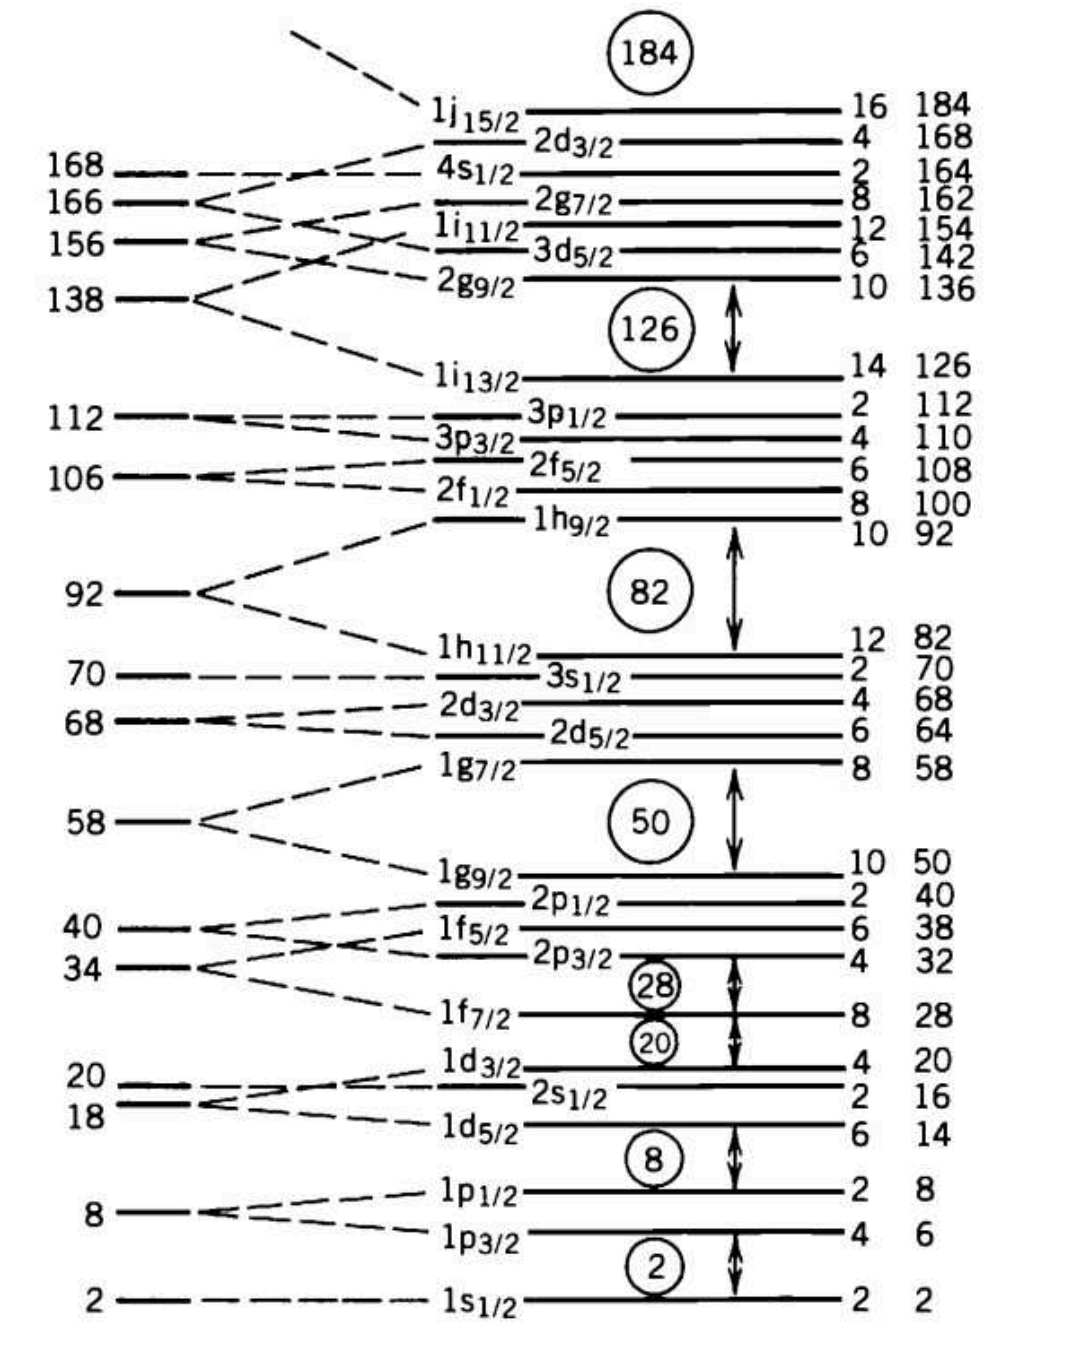
\includegraphics[width=0.5\textwidth]{Images/ShellModel.png}
    \caption{Graphical representation of the shell model solution.}
    \label{fig:shell_model}
\end{figure}


